\documentclass[a4paper,11pt]{article}
\usepackage{graphicx} % Required for inserting images
\usepackage[portuguese]{babel}


\title{BD-PL06}
\author{Eduardo Freitas Fernandes}
\date{2025}

\begin{document}

\maketitle

\noindent \textbf{Exercício 1}\\

\noindent O esquema lógico apresentado está normalizado, mais precisamente na primeira forma normal (\textbf{1FN}). Todas as tabelas têm uma chave primária, os valores de todos os atributos de todas as tabelas são atómicos e não existem grupos de dados repetitivos.\\

\noindent \textbf{Exercício 2}\\

\noindent O esquema apresentado não está na terceira forma normal, então iremos normalizá-lo.\\

\noindent Analisando as dependências funcionais, verificamos que as tabelas \texttt{VendasLivros} e \texttt{ClientesCompras} já estão na segunda forma normal, pois os atributos não-primos dependem da chave primária.\\

\noindent Em relação à tabela \texttt{Livros} verificamos que o atributo \texttt{Categoria\_Nome} não depende da chave primária, logo teremos uma nova tabela (\texttt{Categorias}), e um relacionamento entre \texttt{Vendas e Categorias}.\\

\noindent Olhando para a tabela \texttt{LivrosAutores} vemos que os atributos \texttt{Nome e País} apenas dependem do \texttt{Autor\_Id}, logo teremos que remover esses atributos da tabela e adicionar uma nova tabela, \texttt{Autores}, com esses atributos e o \texttt{Autor\_Id}.\\

\noindent Na tabela \texttt{Vendas} existem duas dependências funcionais que não estão relacionadas com a chave primária da tabela. Os atributos \texttt{Contribuinte e Localidade} dependem do \texttt{Cliente}, logo deveriam estar na tabela dos \texttt{Clientes}. Também vemos que a \texttt{Função} é relativa ao \texttt{Funcionário}, então teremos uma nova tabela, \texttt{Funcionários}, com esse atributo.\\

\noindent Por fim, temos a tabela dos \texttt{Clientes}. O campo \texttt{DesignaçãoProfissão} tem uma dependência transitiva, logo podemos criar uma nova tabela, \texttt{Profissão}, para alocar esse atributo.

\noindent O esquema lógico, após aplicar a normalização até ao terceiro nível, será:

\begin{figure}[h]
    \centering
    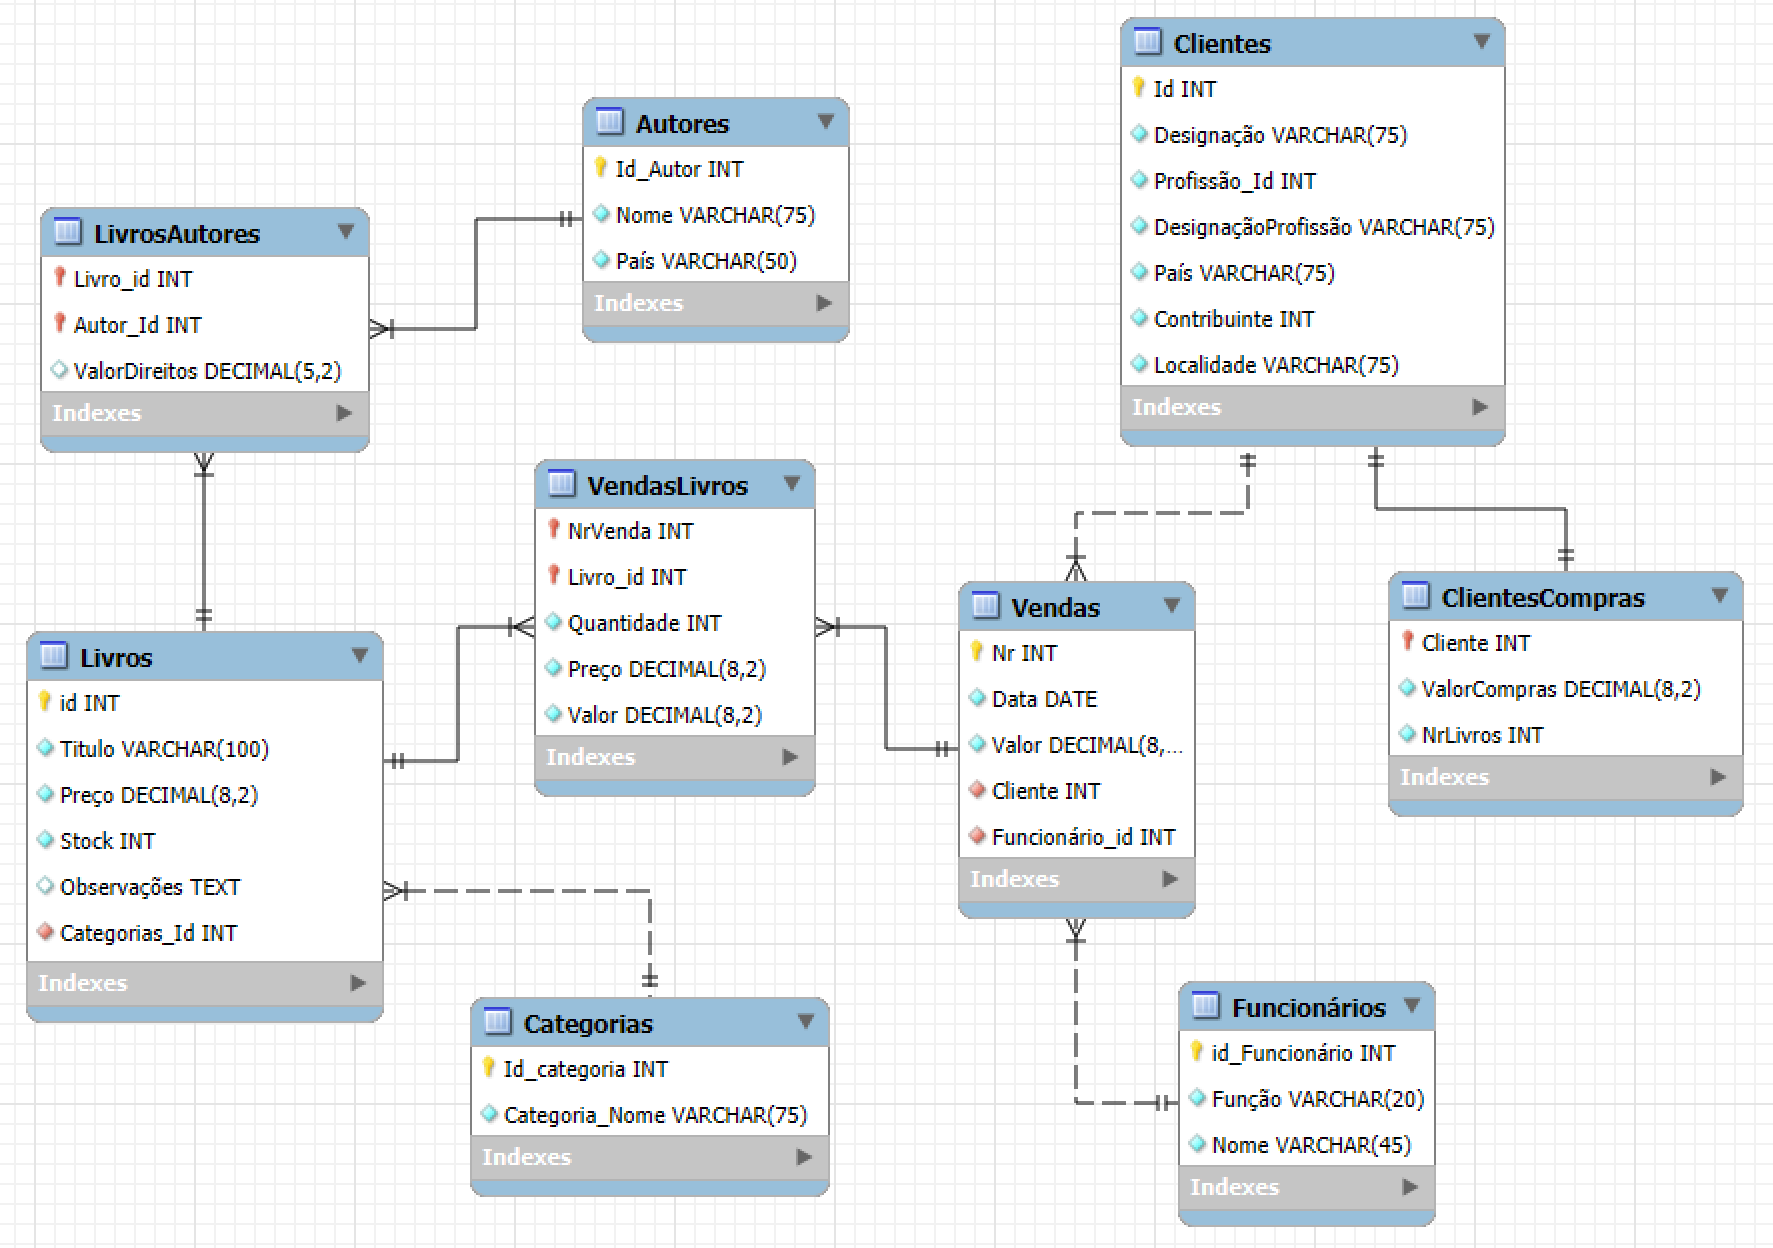
\includegraphics[width=1\linewidth]{imgs/pl06-esquema_logico.png}
    \caption{Esquema Lógico Normalizado (3FN)}
\end{figure}

\noindent \textbf{Exercício 3}\\

\noindent Expressões de Álgebra Relacional para os requisitos apresentados:

\begin{figure}[h]
    \centering
    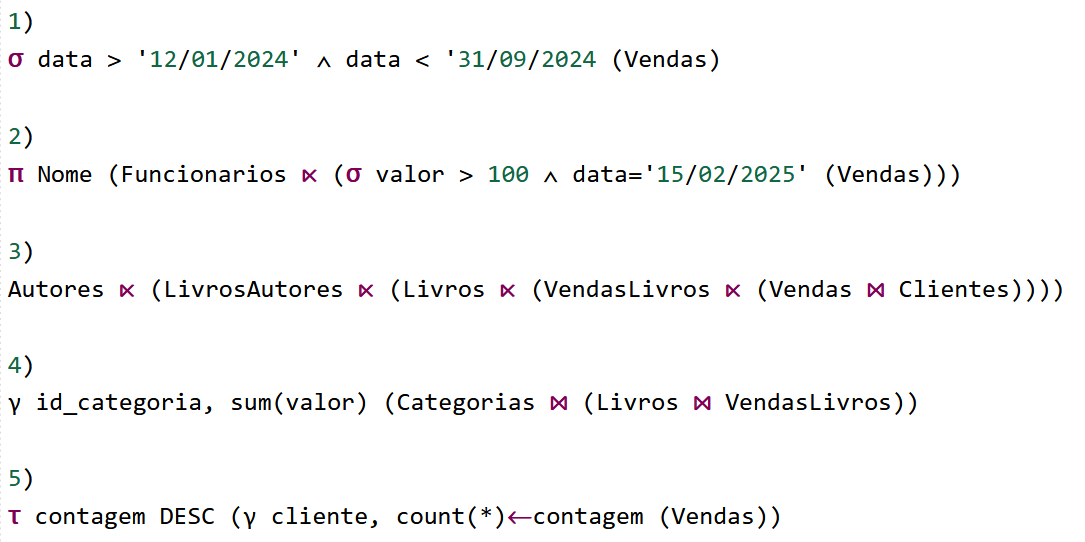
\includegraphics[width=0.75\linewidth]{imgs/exercicio-c.png}
    \caption{Expressões de Álgebra Relacional}
\end{figure}

\end{document}
